%------------------------------------------------------------------------------
%	CAPITOLO 4
%------------------------------------------------------------------------------

\chapter{La paletta della Filomena}
Nelle nostre vecchie case gli operai non erano stati avvelenati dalla propaganda dell'odio di classe, né imposti in ragione delle loro svogliatezze dai sindacati, ma erano un corpo ed un'anima nella famiglia del datore di lavoro. Beati quei tempi di pace in cui anche i nuovi ricchi non erano ancora venuti a spremere il prossimo ed in ispecie gli operai che dovevansi considerare fidati e parte della loro produzione. In casa del Reverendo Don L. M. i suoi operai trovano sempre una buona mezzella\footnote{Fiaschetto di vino da mezzo litro} di vino (non c'erano ancora i daziari a mettere balzelli\footnote{Imposte} al libero trincare), ed un buon fuoco per cuocere la colazione. La mattina i soliti buoni e bravi operai di casa, preparavano un buon fuoco, una mezzetta di vino e si accingevano alla colazione in cucina, scambiando facezie\footnote{Breve racconto costruito su un motto di spirito} con la serva padrona, la buona \index[Personaggi]{Filomena}Filomena.\\
\indent La confidenza tra la \index[Personaggi]{Filomena}Filomena e gli operai era grande, correvano tra di loro facezie, burle e sarcasmi. Messi in sospetto, gli operai, vollero accertarsi che la \index[Personaggi]{Filomena}Filomena non disertasse di notte il letto di castità della zitellona per altro ancora più casto ed escogitarono una burla atroce che refireremo\footnote{Errore dell'autore: si intende 'riferiremo'} in seguito. \\
Filomena, agli operai radunati a tavola per la colazione, chiese:\\
\indent <<Avete preso la palletta del fuoco?>>\\
\indent E gli operai: <<Chi l'ha vista?>>.\\
\indent E così per otto giorni di seguito durò il dialogo al quale però interrogante e gli interrogati sembrava non dessero importanza alcuna. Al nono giorno la domanda ripetuta dalla \index[Personaggi]{Filomena}Filomena si oscurò e comincio ad inalberarsi ... da serva padrona, ma uno degli operai, il più vecchio, con cipiglio ironico mise le cose a punto dicendo:\\
\indent <<La paletta è nel tuo letto e se tu fossi andata a dormire nel tuo letto l'avresti trovata. Invece sei andata a dormire col prete... e noi abbiamo voluto provartelo.>>\\
Come rimasero per questa trovata, la \index[Personaggi]{Filomena}Filomena ed il prete è facile immaginarlo. Il fatto ancora fa ridere i vecchi del paese.

\vspace{0.2cm}
\centerline{\rule{1.5cm}{0.4pt}}
\vspace{0.2cm}

 \begin{figure}[htb]
    \centering
    %\vspace{-0.7cm}
    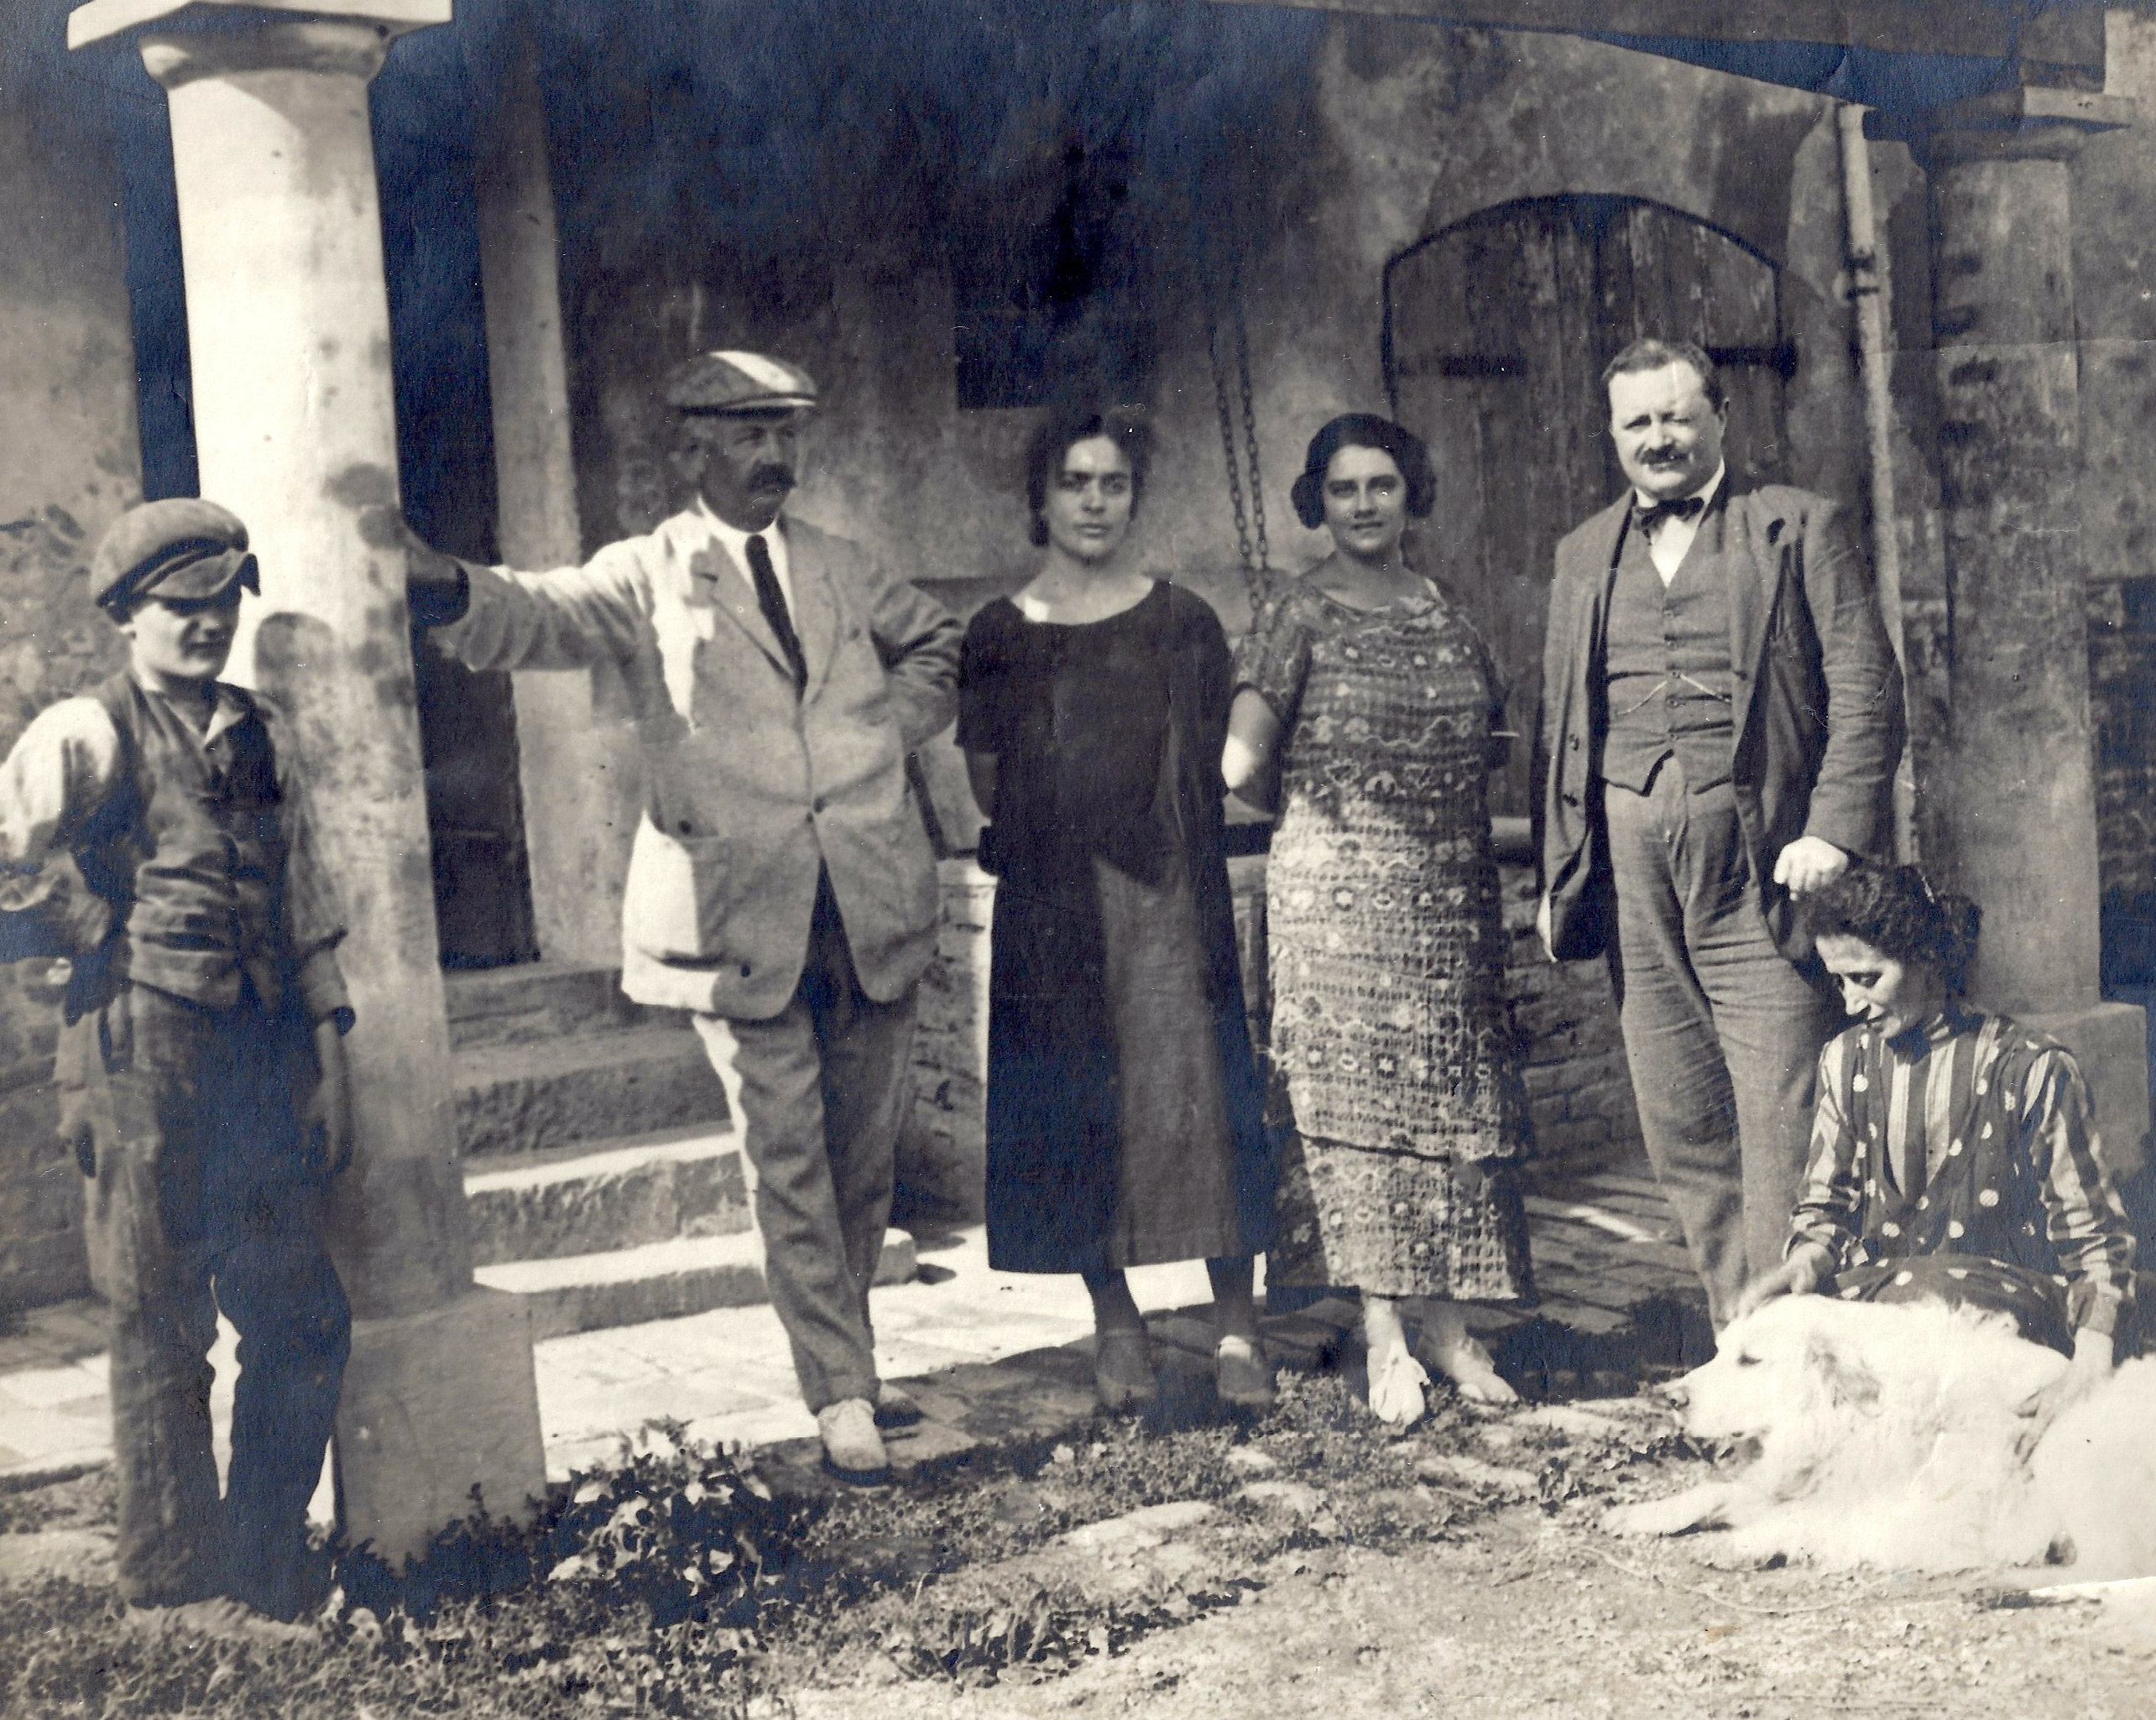
\includegraphics[width=\textwidth]{mingazzigente}
    \caption[Mingazzi con altri (1925)]{\index[Personaggi]{Mingazzi Stefano}Mingazzi a destra e in basso la governante `Ghina' con il cane pastore maremmano di Stefano, `Negar'. A sinistra si riconosce un giovane \index[Personaggi]{Zoli Cesare}Cesare Zoli. Le tre persone al centro non sono state riconosciute. La foto dovrebbe essere stata scattata negli anni '20 quando Mingazzi non era ancora sposato.\index[Personaggi]{Mingazzi Stefano}\label{fig:mingazzigente}}
    %\vspace{-0.3cm}
\end{figure}